% !TeX root = ../main.tex
% 来源：materials/chapter1.pdf，第 5--6 页，1.4 节例题 1--3。

\section{本章例题集}
\label{sec:signals-worked-examples}

\begin{workedexample}[连续时间信号的复合变换]
  \label{ex:signals-affine-triangle}
  已知 $x(t)$ 的波形如\cref{fig:ex-affine-triangle-given} 所示，画出
  \[
    x(3t+6)
    \quad\text{和}\quad
    x(-3t+6)
  \]
  的波形。

  \begin{figure}[htbp]
    \centering
    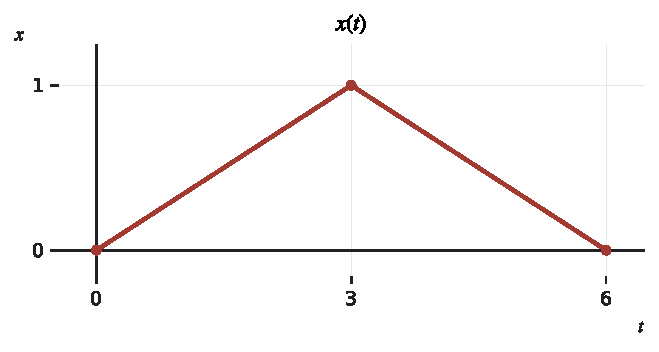
\includegraphics[width=0.52\textwidth]{02-signals/examples/affine-triangle-given.pdf}
    \caption{例题 \ref{ex:signals-affine-triangle} 的已知信号 $x(t)$。}
    \label{fig:ex-affine-triangle-given}
  \end{figure}
\end{workedexample}

\begin{solution}
  先把两个自变量写成便于识别的标准形式：
  \[
    x(3t+6)=x\bigl(3(t+2)\bigr),
    \qquad
    x(-3t+6)=x\bigl(-3(t-2)\bigr).
  \]
  原三角形的关键横坐标为 $0,3,6$，峰值为 $1$。先按翻转、尺度变换、平移的顺序作图：
  \[
    \begin{array}{c|ccc}
      \text{变换步骤}&\text{左端}&\text{峰顶}&\text{右端}\\ \hline
      x(t)&0&3&6\\
      x(3t)\text{：压缩为原来的 }1/3&0&1&2\\
      x(3(t+2))\text{：再左移 }2&-2&-1&0
    \end{array}
  \]
  第二个信号先翻转，再压缩，最后右移：
  \[
    \begin{array}{c|ccc}
      \text{变换步骤}&\text{原左端的位置}&\text{峰顶的位置}&\text{原右端的位置}\\ \hline
      x(-t)&0&-3&-6\\
      x(-3t)&0&-1&-2\\
      x(-3(t-2))&2&1&0
    \end{array}
  \]
  负尺度下，表中按原关键点列出的横坐标从大到小排列；画图时仍按横轴从左到右描点。

  可用关键点映射核对。若原信号中的点位于 $\tau$，则在 $x(at+b)$ 中令
  \[
    at+b=\tau,
    \qquad
    t=\frac{\tau-b}{a}.
  \]
  对 $\tau=0,3,6$，$x(3t+6)$ 的关键点依次变为
  \[
    t=-2,-1,0;
  \]
  对 $x(-3t+6)$，它们依次变为
  \[
    t=2,1,0.
  \]
  两个信号的峰值仍为 $1$，所得波形见\cref{fig:ex-affine-triangle-answer}。

  \begin{figure}[htbp]
    \centering
    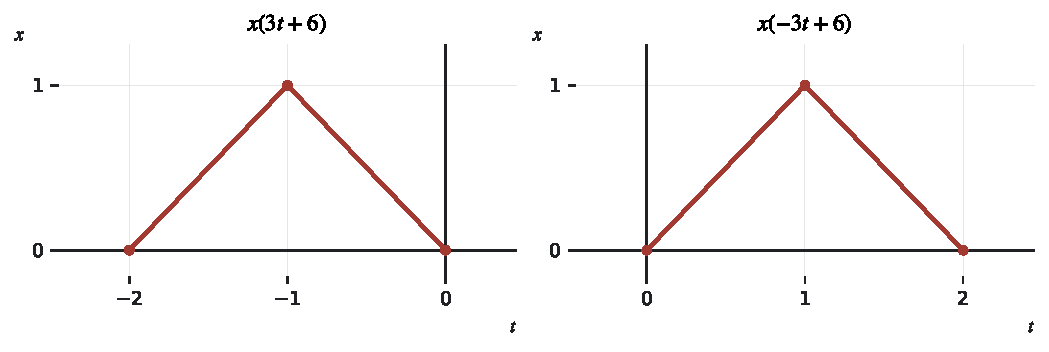
\includegraphics[width=0.82\textwidth]{02-signals/examples/affine-triangle-answer.pdf}
    \caption{例题 \ref{ex:signals-affine-triangle} 的答案。负尺度使第二个信号的关键点顺序反转。}
    \label{fig:ex-affine-triangle-answer}
  \end{figure}
\end{solution}

\begin{technique}
  先化成 $x\bigl(a(t-t_0)\bigr)$，再依次翻转、伸缩和平移，每一步都更新端点与峰顶位置。尺度判断看\red{系数的绝对值}；平移量从括号内的 $t-t_0$ 读取。“左加右减”应在提取尺度系数后使用，最后解 $at+b=\tau$ 核对关键点。
\end{technique}

\begin{workedexample}[由变换后的信号恢复原信号]
  \label{ex:signals-recover-original}
  已知 $y(t)=x(3-2t)$ 的波形如\cref{fig:ex-recover-original-given} 所示，画出 $x(t)$ 的波形。

  \begin{figure}[htbp]
    \centering
    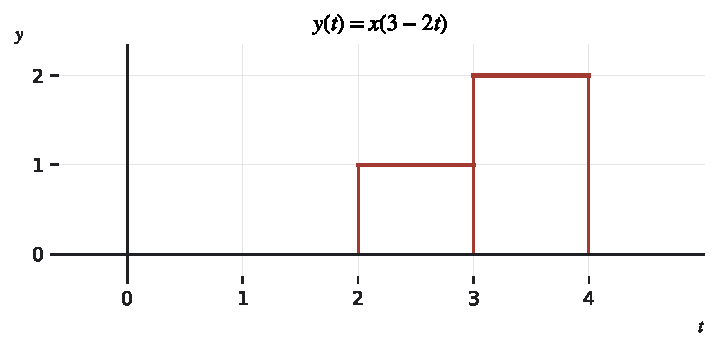
\includegraphics[width=0.56\textwidth]{02-signals/examples/recover-original-given.pdf}
    \caption{例题 \ref{ex:signals-recover-original} 的已知信号 $y(t)=x(3-2t)$。}
    \label{fig:ex-recover-original-given}
  \end{figure}
\end{workedexample}

\begin{solution}
  设
  \[
    u=3-2t,
    \qquad
    t=\frac{3-u}{2}.
  \]
  代回 $y(t)=x(3-2t)$，得到
  \[
    x(u)=y\!\left(\frac{3-u}{2}\right).
  \]
  将哑变量 $u$ 改写成 $t$，即
  \[
    x(t)=y\!\left(\frac{3-t}{2}\right).
  \]
  已知波形的三个边界 $2,3,4$ 分别映射到
  \[
    3-2\times2=-1,
    \qquad
    3-2\times3=-3,
    \qquad
    3-2\times4=-5.
  \]
  因而恢复出的信号为
  \[
    x(t)=
    \begin{cases}
      2,&-5\leq t\leq-3,\\
      1,&-3<t\leq-1,\\
      0,&\text{其他}.
    \end{cases}
  \]
  波形见\cref{fig:ex-recover-original-answer}。

  \begin{figure}[htbp]
    \centering
    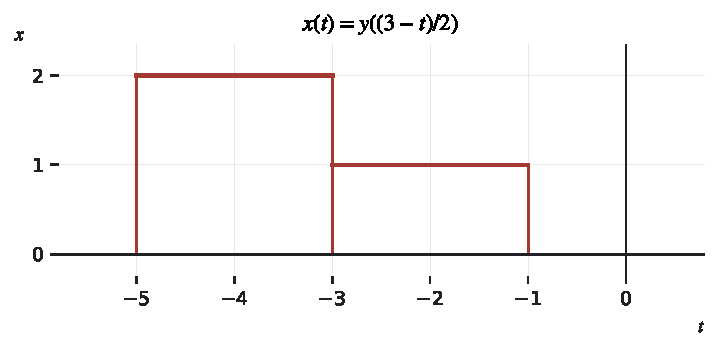
\includegraphics[width=0.56\textwidth]{02-signals/examples/recover-original-answer.pdf}
    \caption{例题 \ref{ex:signals-recover-original} 恢复出的原信号 $x(t)$。}
    \label{fig:ex-recover-original-answer}
  \end{figure}
\end{solution}

\begin{technique}
  已知的是“变换后的信号”而要求原信号时，宜用\red{换元法}：把复合自变量设为新变量，解出旧变量，再代回已知关系。这样可以一次完成反转、尺度和时移，不必逆着猜每一步操作。
\end{technique}

\begin{workedexample}[离散时间序列的平移与反转]
  \label{ex:signals-discrete-transform}
  已知序列 $x[n]$ 如\cref{fig:ex-discrete-transform-given} 所示，其非零样值为
  \[
    x[-2]=\frac12,
    \quad x[-1]=-\frac12,
    \quad x[0]=x[1]=x[2]=x[3]=1.
  \]
  画出 $x[n-3]$ 和 $x[4-n]$ 的波形。

  \begin{figure}[htbp]
    \centering
    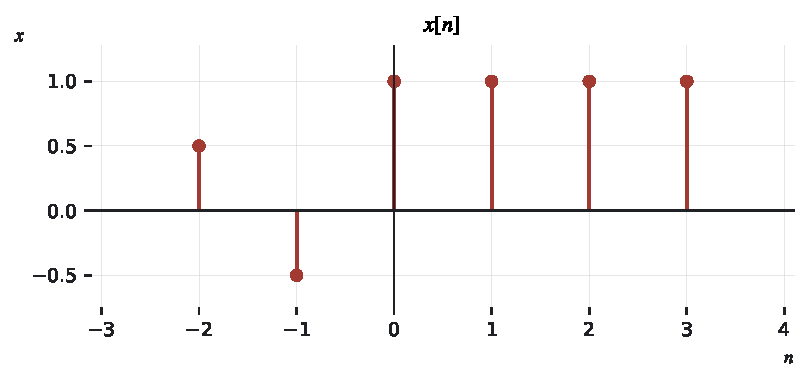
\includegraphics[width=0.62\textwidth]{02-signals/examples/discrete-transform-given.pdf}
    \caption{例题 \ref{ex:signals-discrete-transform} 的已知序列 $x[n]$。}
    \label{fig:ex-discrete-transform-given}
  \end{figure}
\end{workedexample}

\begin{solution}
  对 $x[n-3]$，令 $n-3=k$，所以原来位于 $k$ 的样值移到 $n=k+3$。因此
  \[
    x[n-3]\ne0
    \quad\text{仅当}\quad
    n=1,2,3,4,5,6,
  \]
  相应幅值依次为
  \[
    \frac12,-\frac12,1,1,1,1.
  \]

  对 $x[4-n]$，令 $4-n=k$，所以原来位于 $k$ 的样值移到 $n=4-k$。相应地，$n=1,2,3,4$ 处的值为 $1$，$n=5$ 处为 $-1/2$，$n=6$ 处为 $1/2$。两组结果见\cref{fig:ex-discrete-transform-answer}。
  \[
    \begin{array}{c|rrrrrr}
      \text{原下标 }k&-2&-1&0&1&2&3\\ \hline
      x[k]&1/2&-1/2&1&1&1&1\\
      x[n-3]\text{ 中的位置 }n=k+3&1&2&3&4&5&6\\
      x[-n]\text{ 中的位置 }n=-k&2&1&0&-1&-2&-3\\
      x[4-n]\text{ 中的位置 }n=4-k&6&5&4&3&2&1
    \end{array}
  \]
  最后一行也可由上一行每个位置加 $4$ 得到，即先反转，再右移 $4$。

  \begin{figure}[htbp]
    \centering
    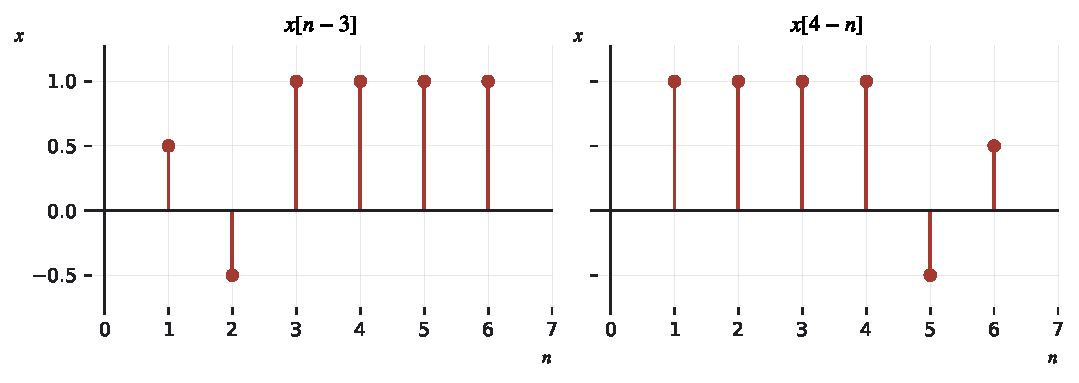
\includegraphics[width=0.84\textwidth]{02-signals/examples/discrete-transform-answer.pdf}
    \caption{例题 \ref{ex:signals-discrete-transform} 的答案。离散序列只在整数位置取值。}
    \label{fig:ex-discrete-transform-answer}
  \end{figure}
\end{solution}

\begin{technique}
  离散信号与连续信号使用同一个关键点映射方法，但应逐点处理。把每个非零样值记成 $(k,x[k])$，解出它在新序列中的整数位置，幅值原样搬过去；最后检查是否漏点、是否误把相邻样值连成连续曲线。
\end{technique}
